\documentclass{puzz}
\usepackage{longtable}
\usepackage{tabu}
\usepackage{pgffor}

\makeatletter
\newcommand*{\n}[1]{%
    \setlength{\skip@}{1em}%
    \vrule \@height 8mm \@width\z@
    \nobreak \leaders\hrule \@height .2\p@ \hskip\skip@
    \nobreak
    \hskip -\skip@
    \divide\skip@\tw@
    \hskip\skip@
    \makebox[\z@][c]{\raisebox{-1.1ex}[\z@][\z@]{\tiny #1}}%
    \nobreak\hskip\skip@
    \kern\p@ % in case a punctuation follows
}

\newcommand*{\ns}[1]{%
    \foreach \x in {#1} {\n{\x}\ }
}
\makeatother

\begin{document}
\puzztitle{Puzzle 3: Time Acrostic}
\vspace{-0.2ex}
\begin{center}
    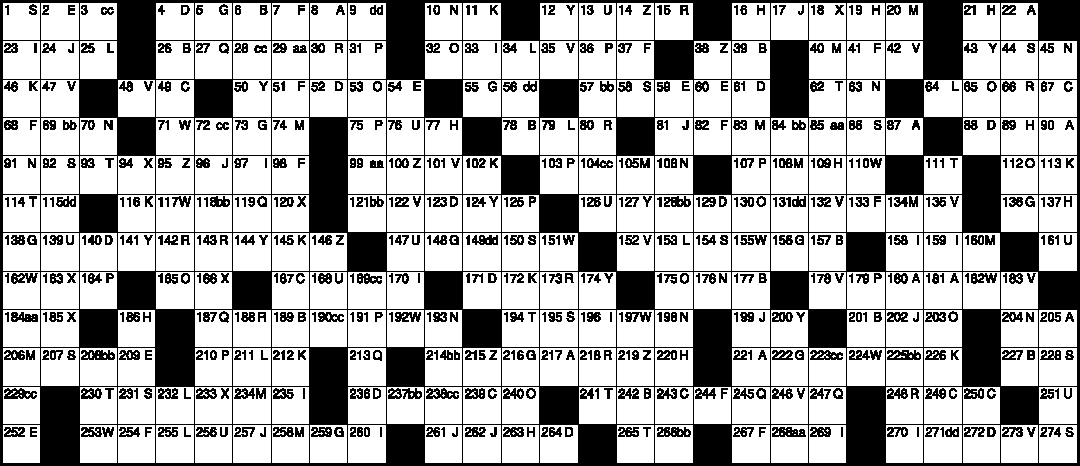
\includegraphics[width=\textwidth]{tw-data/time-graphic.pdf}
\end{center}

\begin{longtabu}{>{\footnotesize}p{12pt} >{\footnotesize}X >{\small}p{187pt}}
    A. & It keeps what this quotation's author is looking for. & \ns{221,8,217,87,22,90,181,180,205} \\
    B. & In accordance with clue E & \ns{227,26,39,242,177,201,78,6,189,157} \\
    C. & Fact-checked, maybe & \ns{249,250,49,67,167,243,239} \\
    D. & Disaster & \ns{88,272,129,52,264,171,236,123,4,61,140} \\
    E. & Topic taught in HASS & \ns{54,209,2,59,60,252} \\
    F. & Creature that looks\dots{} different\dots{} under the full moon. & \ns{254,37,7,68,244,267,41,82,133,51,98} \\
    G. & Orbital point closest to the Sun & \ns{138,156,216,55,148,73,5,136,222,259} \\
    H. & Technique used by Markov Chain Monte Carlo methods & \ns{77,186,220,21,89,137,19,263,109,16} \\
    I. & ``August: \rule{30pt}{0.8pt} \rule{30pt}{0.8pt}'' (Pulitzer-winning play) & \ns{33,235,196,260,269,97,158,159,23,170,270} \\
    J. & Mother of Shelob & \ns{202,96,81,24,262,199,261,17,257} \\
    \clearpage \\
    K. & House named after founder Salazar & \ns{116,46,102,226,113,11,212,172,145} \\
    L. & Caricaturist Lautrec & \ns{25,211,79,34,153,232,64,255} \\
    M. & Stretch of what this quotation’s author is looking for. & \ns{258,108,40,83,105,160,234,206,20,134,74} \\
    N. & London-set novel by Neil Gaiman & \ns{193,198,91,70,45,10,176,63,204,106} \\
    O. & “There are 400 CS majors at Mines”, e.g. & \ns{32,175,165,203,130,240,112,65,53} \\
    P. & Snack favored by Eleven of “Stranger Things” & \ns{164,125,31,107,103,191,210,75,36,179} \\
    Q. & Indict & \ns{213,187,119,245,247,27} \\
    R. & Gives more of what this quotation’s author is looking for, perhaps & \ns{80,188,248,30,143,173,218,66,15,142} \\
    S. & They keep track of what this quotation’s author is looking for.  & \ns{150,58,154,231,228,44,195,92,1,86,207,274} \\
    T. & Oft-derided -- yet delicious -- pizza & \ns{230,265,62,241,194,114,111,93} \\
    U. & The titular character of “Free Willy”, for one.  & \ns{76,139,126,13,147,168,251,161,256} \\
    V. & Demand from Audrey of “Little Shop of Horrors” & \ns{152,101,35,47,122,42,135,246,183,178,48,132,273} \\
    W. & 1967 hit from The Doors & \ns{117,192,197,151,71,155,110,253,162,182,224} \\
    X. & Located elsewhere & \ns{18,163,185,233,94,166,120} \\
    Y. & Winter trek equipment & \ns{50,124,127,43,200,12,144,174,141} \\
    Z. & Some picaresque characters & \ns{38,100,219,215,14,95,146} \\
    aa. & Purchase from the Mines Geology Museum, perhaps & \ns{85,29,184,99,268} \\
    bb. & Scientist who formalized what this quotation’s author is looking for.  & \ns{118,266,121,84,214,225,208,57,69,237,128} \\
    cc. & Black-and-white Black Mirror episode & \ns{223,3,190,238,28,72,104,169,229} \\
    dd. & Wesley Crusher, e.g.  & \ns{271,56,9,149,131,115} \\
\end{longtabu}

For your answer on the website, enter:

Name of the quote's author, followed by title of the quote's source (as spelled
out by the first letter of each answer, A-dd), without any spaces.
\end{document}
% o"*pf.li &jdd:s/ /,/g
I& \ns{A} \\k$J
